%%%%%%%%%%%%%%%%%%%%%%%%%%%%%%%%%%%%%%%%%%%%%%%%%%%%%%%%%%%%%%%%%
% MUW Presentation
% LaTeX Template
% Version 1.0 (27/12/2016)
%
% License:
% CC BY-NC-SA 4.0 (http://creativecommons.org/licenses/by-nc-sa/3.0/)
%
% Created by:
% Nicolas Ballarini, CeMSIIS, Medical University of Vienna
% nicoballarini@gmail.com
% http://statistics.msi.meduniwien.ac.at/
%
% Customized for UAH by:
% David F. Barrero, Departamento de Automática, UAH
%%%%%%%%%%%%%%%%%%%%%%%%%%%%%%%%%%%%%%%%%%%%%%%%%%%%%%%%%%%%%%%%%

\documentclass[10pt,compress]{beamer} % Change 10pt to make fonts of a different size
\mode<presentation>

\usepackage[spanish]{babel}
\usepackage{fontspec}
\usepackage{tikz}
\usepackage{etoolbox}
\usepackage{xcolor}
\usepackage{xstring}
\usepackage{listings}

% Custom pñackages
\usepackage{multicol}
\usepackage{tikz}
\usetikzlibrary{matrix,chains,positioning,decorations.pathreplacing,arrows,shapes}

\usetheme{UAH}
\usecolortheme{UAH}
\setbeamertemplate{navigation symbols}{} 
\setbeamertemplate{caption}[numbered]

%%%%%%%%%%%%%%%%%%%%%%%%%%%%%%%%%%%%%%%%%%%%%%%%%%%%%%%%%%%%%%%%%
%% Presentation Info
\title[Python for videogames]{Python for videogames}
\author{\asignatura\\\carrera}
\institute{}
\date{Departamento de Automática}
%%%%%%%%%%%%%%%%%%%%%%%%%%%%%%%%%%%%%%%%%%%%%%%%%%%%%%%%%%%%%%%%%


%%%%%%%%%%%%%%%%%%%%%%%%%%%%%%%%%%%%%%%%%%%%%%%%%%%%%%%%%%%%%%%%%
%% Descomentar para habilitar barra de navegación superior
\setNavigation
%%%%%%%%%%%%%%%%%%%%%%%%%%%%%%%%%%%%%%%%%%%%%%%%%%%%%%%%%%%%%%%%%

%%%%%%%%%%%%%%%%%%%%%%%%%%%%%%%%%%%%%%%%%%%%%%%%%%%%%%%%%%%%%%%%%
%% Configuración de logotipos en portada
%% Opacidad de los logotipos
\newcommand{\opacidad}{1}
%% Descomentar para habilitar logotipo en pié de página de portada
%\renewcommand{\logoUno}{Images/isg.png}
%% Descomentar para habilitar logotipo en pié de página de portada
%\renewcommand{\logoDos}{Images/CCLogo.png}
%% Descomentar para habilitar logotipo en pié de página de portada
\renewcommand{\logoTres}{Images/ALogo.png}
%% Descomentar para habilitar logotipo en pié de página de portada
%\renewcommand{\logoCuatro}{Images/ELogo.png}
%%%%%%%%%%%%%%%%%%%%%%%%%%%%%%%%%%%%%%%%%%%%%%%%%%%%%%%%%%%%%%%%%

%%%%%%%%%%%%%%%%%%%%%%%%%%%%%%%%%%%%%%%%%%%%%%%%%%%%%%%%%%%%%%%%%
%% FOOTLINE
%% Comment/Uncomment the following blocks to modify the footline
%% content in the body slides. 


%% Option A: Title and institute
\footlineA
%% Option B: Author and institute
%\footlineB
%% Option C: Title, Author and institute
%\footlineC
%%%%%%%%%%%%%%%%%%%%%%%%%%%%%%%%%%%%%%%%%%%%%%%%%%%%%%%%%%%%%%%%%

\begin{document}

%%%%%%%%%%%%%%%%%%%%%%%%%%%%%%%%%%%%%%%%%%%%%%%%%%%%%%%%%%%%%%%%%
% Use this block for a blue title slide with modified footline
{\titlepageBlue
    \begin{frame}
        \titlepage
    \end{frame}
}

\institute{\asignatura}

\begin{frame}[plain]{}
	\begin{block}{Objectives}
		\begin{enumerate}
		\item Understand the relevance to use modules and packages.
		\item Install some widely used Python packages.
		\item First contact with Arcade.
		\end{enumerate}
	\end{block}

	\begin{block}{Bibliography}
		\begin{itemize}
			\item The Python Tutorial. \textit{Chapter 6: Modules}. \href{https://docs.python.org/3/tutorial/modules.html}{(Link)}
			\item Paul Vincent Craven. \textit{Easy 2D game creation with Arcade}. \href{https://speakerdeck.com/pycon2018/paul-vincent-craven-easy-2d-game-creation-with-arcade}{(Link)}
			\item Paul Vincent Craven. \textit{Learn to Program with Arcade}. \href{https://learn.arcade.academy/en/latest/}{(Link)}
		\end{itemize}
	\end{block}
\end{frame}

{
\disableNavigation{white}
\begin{frame}[shrink]{Table of Contents}

 	\frametitle{Table of Contents}
  	\begin{multicols}{2}
  		\tableofcontents
    	\end{multicols}

 %\frametitle{Table of Contents}
 %\tableofcontents
  % You might wish to add the option [pausesections]
\end{frame}
}

\section{Introduction}
\begin{frame}{Introduction}
		\begin{block}{Why modules?}
			\begin{itemize}
			\item \textbf{Main function}: Organization.
			\item \textbf{Reuse}: To provide software solutions, that have been proven to work, to solve similar problems.
			\end{itemize}
		\end{block}
\end{frame}

\section{Modules}

\subsection{Using modules}
\begin{frame}{Using modules}{Creation and Implementation}
	\vspace{-0.2cm}
	A module is just a Python script with \texttt{.py} extension
	\vspace{-0.2cm}
	%creo que está mal fibo.py
	\begin{exampleblock}{fibo.py}
	\vspace{-0.2cm}
	\lstinputlisting[basicstyle=\scriptsize,numbers=left]{code/fibo.py}
	\vspace{-0.2cm}
	\end{exampleblock}
\end{frame}

\begin{frame}[fragile]{Using modules}{How do I use them? (I)}
	\begin{block}{}
	\begin{verbatim}
>>> import fibo
>>> fibo.fib(1000)
1 1 2 3 5 8 13 21 34 55 89 144 233 377 610 987
>>> fibo.fib2(100)
[1, 1, 2, 3, 5, 8, 13, 21, 34, 55, 89]
>>> fibo.__name__
'fibo'
>>> fib = fibo.fib
>>> fib(100)
1 1 2 3 5 13 21 34 55 89
\end{verbatim}
	\vspace{-0.2cm}
	\end{block}
\end{frame}

\begin{frame}[fragile]{Using modules}{How do I use them?  (II)}
	A module can import other modules
		\begin{itemize}
		\item Name conflicts may arise: Each module has a symbol table
		\item It means you should invoke it as \texttt{modname.itemname}
		\end{itemize}
 	It is possible to import items directly
		\begin{itemize}
		\item \texttt{from module import name1, name2}
		\item \texttt{from module import *}
		\item It uses the global symbol table (no need to use the modname)
			\end{itemize}
	
	\begin{exampleblock}{}
	\begin{verbatim}
>>> from fibo import fib, fib2
>>> fib(100)
1 1 2 3 5 8 13 21 34 55 89 144 233 377 610 987
\end{verbatim}
	\end{exampleblock}
\end{frame}

\begin{frame}[fragile]{Using modules}{How do I use them?  (III)}
	\vspace{-0.2cm}
	\begin{block}{List zip file contents (file.zip must exist. Open in read mode)}
	\vspace{-0.2cm}
	\lstinputlisting[numbers=left]{code/zip.py}
	\vspace{-0.2cm}
	\end{block}
	
	\vspace{-0.2cm}
	\centering \footnotesize{Several examples here: \url{http://pymotw.com/2/PyMOTW-1.132.pdf}}
\end{frame}

\subsection{Executing modules}

\begin{frame}{Executing modules}{Modules as scripts (I)}
	When a module is imported, its statements are executed
		\begin{itemize}
		\item It declares functions, classes, variables ...
		\item ... and also executes code
		\item It serves to initialize the module
		\end{itemize}
	Very useful to use modules as programs and libraries
\end{frame}

\begin{frame}[shrink,plain,fragile]{Executing modules}{Modules as scripts (II)}
    \small
	\vspace{-0.3cm}
	\begin{exampleblock}{fibo2.py}
	\vspace{-0.2cm}
	\lstinputlisting[numbers=left]{code/fibo2.py}
	\vspace{-0.2cm}
	\end{exampleblock}

	\vspace{-0.5cm}
	\begin{columns}
 	   \column{0.5\textwidth}
	\begin{exampleblock}{}
	\vspace{-0.2cm}
	\begin{verbatim}
    (In Linux console)
$ python3 fibo2.py 50
1 1 2 3 5 8 13 21 34
\end{verbatim}
	\vspace{-0.2cm}
	\end{exampleblock}

 	   \column{0.5\textwidth}
	\begin{exampleblock}{}
	\vspace{-0.2cm}
	\begin{verbatim}
    (In Python interpreter)
>>> import fibo2
>>> fibo2.fib(50)
1 1 2 3 5 8 13 21 34
\end{verbatim}
	\vspace{-0.2cm}
	\end{exampleblock}

    \end{columns}
\end{frame}

\subsection{Content of a module}

\begin{frame}[fragile]{Content of a module}{The dir() function}
	Very usefull to get an insight to a module
	\begin{itemize}
		\item It returns the names defined in a module
		\item Without arguments, it returns your names
	\end{itemize}
	\begin{exampleblock}{}
	\begin{verbatim}
>>> import fibo, sys
>>> dir(fibo)
['__name__', 'fib', 'fib2']
>>> dir()
['__builtins__', ... , '__spec__']
>>> variable = 'Hello'
>>> dir()
['__builtins__', ... , '__spec__', 'variable']
\end{verbatim}
	\vspace{-0.2cm}
	\end{exampleblock}
\end{frame}

\section{Packages}
\subsection{Package concept}
\begin{frame}{Packages}{Package concept (I)}
		If a module gets too big, many problems arise
			\begin{itemize}
			\item Name collisions
			\item It is good to organize modules in a bigger structure: \textit{Packages}
			\end{itemize}
		Packages can be seen as ``dotted module names''
			\begin{itemize}
			\item It is just a module that contains more modules
			\item Make life easier in big proyects
			\item The name \texttt{A.B} designates a submodule \texttt{B} in a package named \texttt{A}
			\end{itemize}
		Must contain a \texttt{\_\_init\_\_.py} file in the root directory
			\begin{itemize}
			\item Executed when the package is imported for the first time
			\end{itemize}
\end{frame}

\begin{frame}[shrink,plain]{Packages}{Package concept (II)}
	\centering \textit{Sound module structure}
	\lstinputlisting{code/module.txt}
\end{frame}

\subsection{Importing a package}
\begin{frame}{Packages}{Importing a package (I)}
	\centering{\alert{Ways to use a package}}\\
	\bigskip
	\begin{flushleft}
	Import an individual module
		\begin{itemize}
		\item \texttt{import sound.effects.echo}
		\item Use function as \texttt{sound.effects.echo.echofilter(input, output)}
		\end{itemize}
	Alternative way to import an individual module
		\begin{itemize}
		\item \texttt{from sound.effects import echo}
		\item Use function as \texttt{echo.echofilter(input, output)}
		\end{itemize}
	Alternative way to import an individual module
		\begin{itemize}
		\item \texttt{from sound.effects.echo import echofilter}
		\item Use function as \texttt{echofilter(input, output)}
		\end{itemize}
	\end{flushleft}
\end{frame}

\begin{frame}{Packages}{Importing a package (II)}
	Imagine we run \texttt{from sound import *}
		\begin{itemize}
		\item In theory, it would import the whole package
		\item In practice, it would take too much time
		\end{itemize}
	There is a convention to avoid waste of resources
		\begin{itemize}
		\item There may be a variable \texttt{\_\_all\_\_} defined in \texttt{\_\_init\_\_}
		\item \texttt{\_\_all\_\_} contains modules to be imported
		\end{itemize}

	\begin{block}{sounds/effects/\_\_init\_\_.py}
	\vspace{-0.2cm}
	\lstinputlisting{code/package.py}
	\vspace{-0.2cm}
	\end{block}
\end{frame}

\subsection{Installing packages}
\begin{frame}[fragile]{Packages}{Installing packages (I)}
	Command-line automatic tool: \texttt{pip} (sometimes \texttt{pip3})
		\begin{itemize}
			\item Very similar to \texttt{apt-get} in Linux
		\end{itemize}

	\begin{block}{pip usage (from OS terminal)}
	\vspace{-0.2cm}
	\begin{verbatim}
$ python -m pip install SomePackage
\end{verbatim}
or
	\begin{verbatim}
$ pip install SomePackage
\end{verbatim}
	\vspace{-0.2cm}
\end{block}

	\begin{exampleblock}{}
	\vspace{-0.2cm}
	\begin{verbatim}
$ pip install Pillow
\end{verbatim}
	\vspace{-0.2cm}
\end{exampleblock}
    List of dependences in \texttt{requirements.txt}
\end{frame}

\begin{frame}[fragile]{Packages}{Installing packages (II)}
	    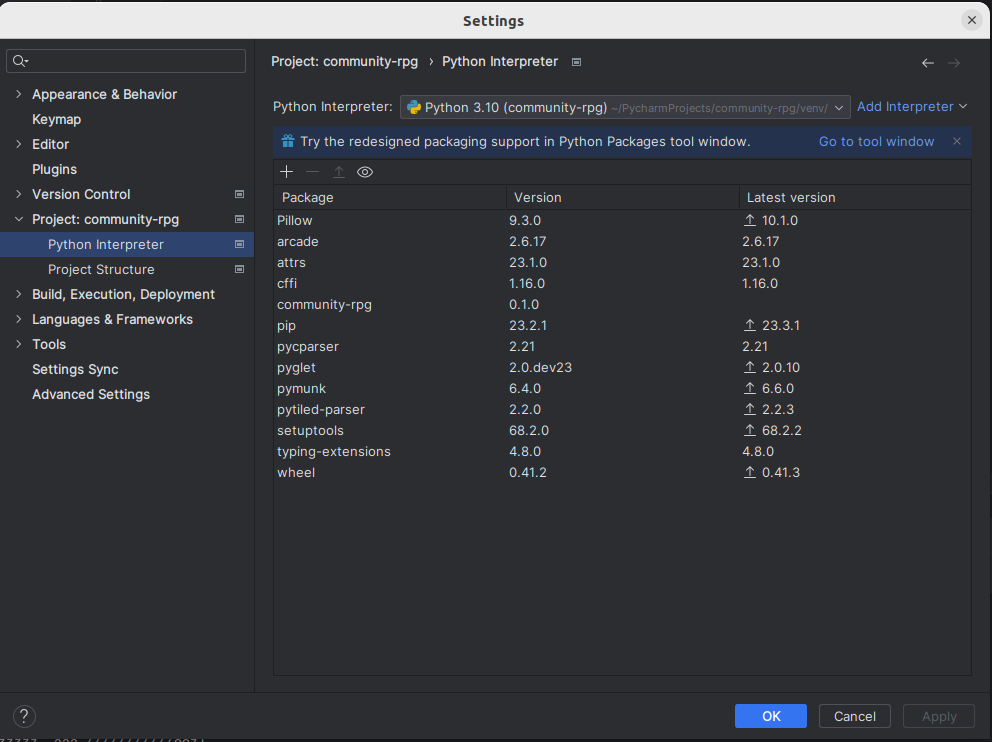
\includegraphics[width=0.8\linewidth]{figs/packages}
\end{frame}

\section{Other cool code examples}

\subsection{Example 1: Open a web browser}
\begin{frame}{Cool code examples}{Example 1: Open a web browser}
	\vspace{-0.2cm}
	\begin{block}{browser.py}
	\vspace{-0.2cm}
	\lstinputlisting{code/brower.py}
	\vspace{-0.2cm}
	\end{block}
\end{frame}

\subsection{Example 2: Create a thumbnail}
\begin{frame}[plain]{Cool code examples}{Example 2: Create a thumbnail}
	\begin{columns}
 	   \column{.60\textwidth}

		\vspace{-0.2cm}
		\begin{block}{thumbnail.py}
		\vspace{-0.2cm}
		\lstinputlisting{code/thumbnail.py}
		\vspace{-0.2cm}
		\end{block}

		

  		\column{.50\textwidth}
		\vspace{-0.2cm}
		\centering 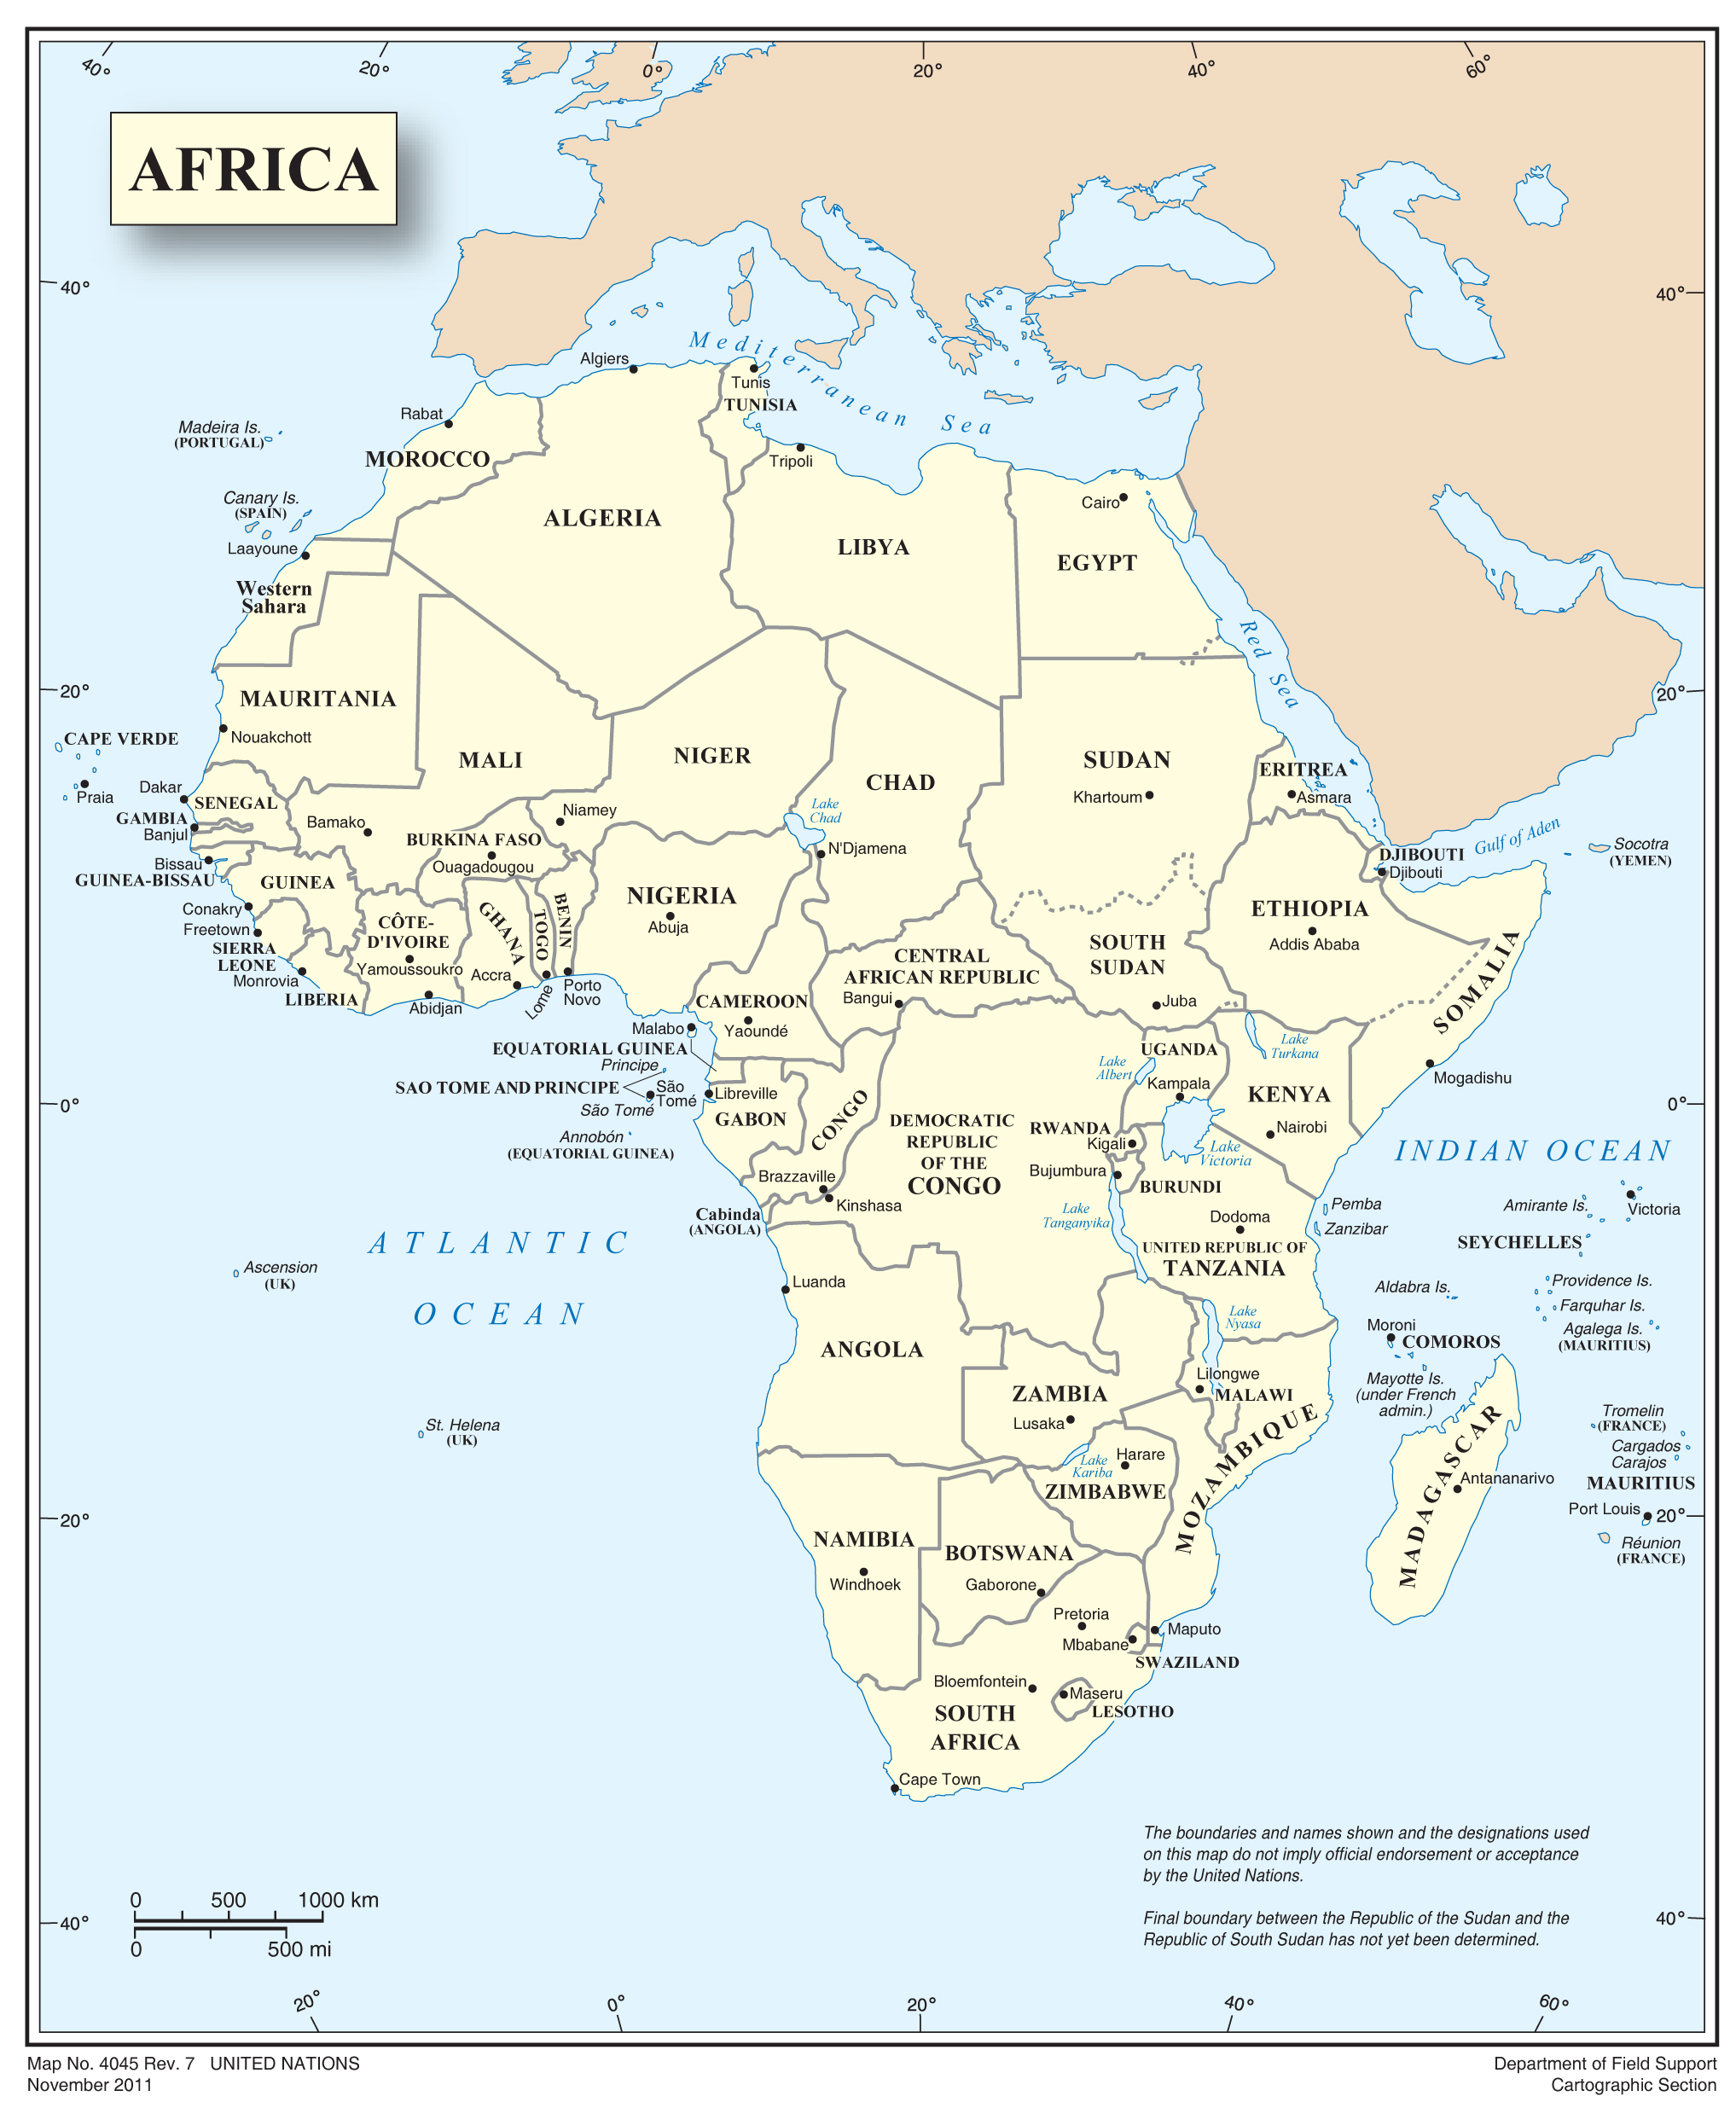
\includegraphics[width=\linewidth]{figs/africa.jpg}\\
	 	\texttt{africa.jpg}
	\end{columns}
		\vspace{-0.2cm}
	\centering \tiny{\href{http://www.pythonforbeginners.com/gui/how-to-use-pillow}{(Source)}}
\end{frame}

\subsection{Example 3: Send an email with Gmail}
\begin{frame}{Cool code examples}{Example 4: Send an email with Gmail}
	\begin{columns}
 	   \column{1.1\textwidth}
		\vspace{-0.2cm}
		\begin{block}{gmail.py}
		\vspace{-0.2cm}
		\lstinputlisting{code/gmail.py}
		\end{block}
	\end{columns}

	\centering \tiny{\href{http://www.pythonforbeginners.com/code-snippets-source-code/using-python-to-send-email/}{(Source)}}
\end{frame}

\begin{frame}{Modules}{Example 4: Plot}
	\begin{columns}
 	   \column{.60\textwidth}

		\vspace{-0.2cm}
		\begin{exampleblock}{plot.py}
		\vspace{-0.2cm}
		\lstinputlisting{code/plot.py}
		\vspace{-0.2cm}
		\end{exampleblock}

  		\column{.50\textwidth}
		\vspace{-0.2cm}
		\centering 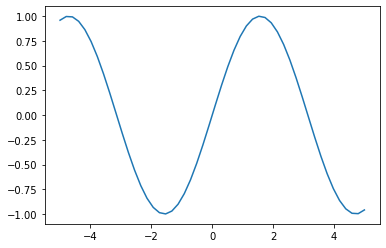
\includegraphics[width=\linewidth]{figs/plot.png}\\
	\end{columns}
		\vspace{-0.2cm}
\end{frame}

\begin{frame}{Modules}{Example 5: Arcade}
	\begin{columns}
 	   \column{0.80\textwidth}

		\vspace{-0.2cm}
		\begin{exampleblock}{arcade.py}
		\vspace{-0.2cm}
		\lstinputlisting{code/arcade.py}
		\vspace{-0.2cm}
		\end{exampleblock}

  		\column{.40\textwidth}
		\vspace{-0.2cm}
		\centering 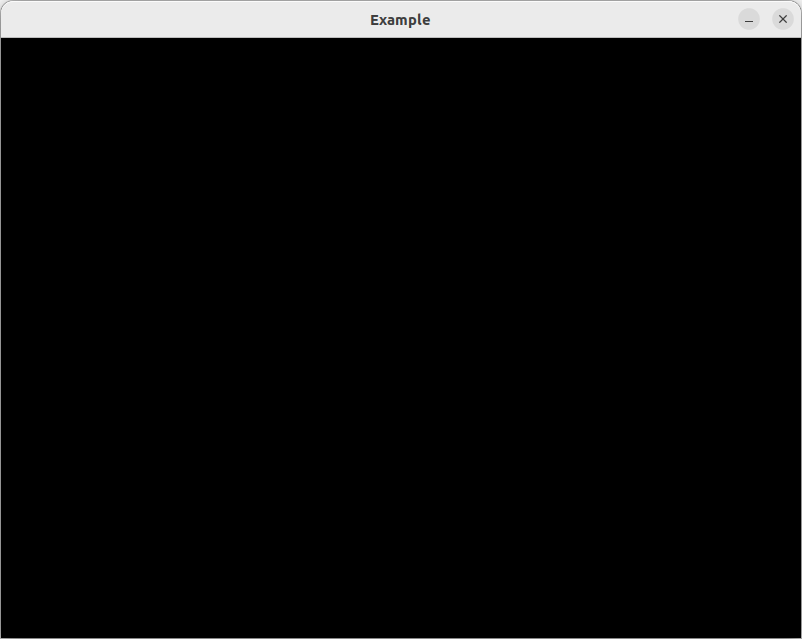
\includegraphics[width=\linewidth]{figs/window.png}\\
		\vspace{-0.2cm}
	\end{columns}

	\begin{itemize}
		\item \href{https://api.arcade.academy/en/latest/arcade.html}{(API documentation)}
		\item \href{https://github.com/pythonarcade/arcade/tree/development}{(Arcade source code)}
	\end{itemize}
\end{frame}

\section{Virtual environments}

\begin{frame}{Virtual environments}
	\begin{columns}
 	   \column{0.50\textwidth}
            Versioning is problematic
            \begin{itemize}
                \item Python version (2.x, 3.x)
                \item Packages version
            \end{itemize}
            Solution: \alert{virtual environment}
            \begin{itemize}
                \item Self-contained directory with a Python installation
                \item Particular version of Python and packages
            \end{itemize}
        	Different solutions
            \begin{itemize}
                \item venv
                \item conda
            \end{itemize}
            Great tool with \texttt{requirements.txt}
 	   \column{0.50\textwidth}
	        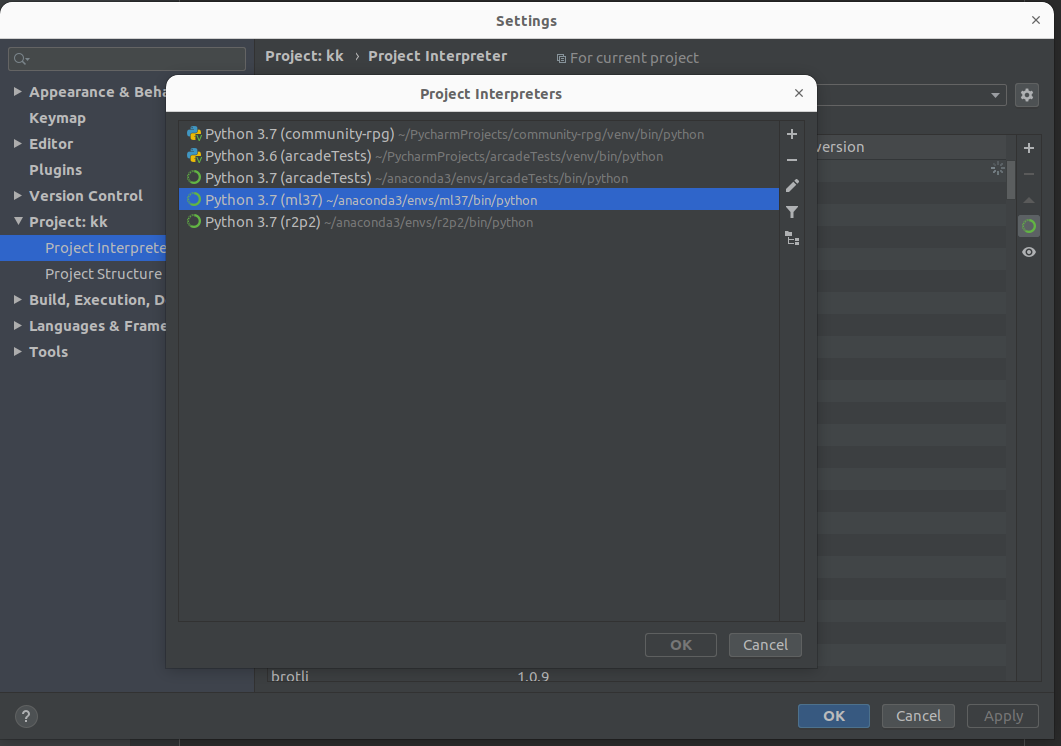
\includegraphics[width=\linewidth]{figs/venv.png}\\
	\end{columns}
\end{frame}

\section{Arcade}
\subsection{Introduction}

\begin{frame}{Arcade}{Introduction}
	\begin{columns}
 	   \column{0.60\textwidth}
		Arcade is an easy-to-use 2D motor engine (i.e. a Python package)
            \begin{itemize}
		\item Created by Paul Vincent Craven
                \item Based on Python
                \item More or less painless game development
                \item Didactic
                \item Free software
            \end{itemize}

        	Requires
            \begin{itemize}
                \item Python 3.6+
                \item OpenGL capable hardware
            \end{itemize}

            Dependences
            \begin{itemize}
                \item Pyglet - Mutimedia library for Python
            \end{itemize}

 	   \column{0.30\textwidth}
            
\includegraphics[width=\linewidth]{figs/arcade-logo}\\
    		\href{http://arcade.academy}{(Arcade web site)}
 	   \column{0.10\textwidth}
	\end{columns}
\end{frame}

\subsection{Open a Window}
\begin{frame}{Arcade}{Open a Window (I)}
	\begin{columns}
 	   \column{0.80\textwidth}
		\vspace{-0.2cm}
		\begin{exampleblock}{arcade.py}
		\vspace{-0.2cm}
		\lstinputlisting[numbers=left]{code/arcade.py}
		\vspace{-0.2cm}
		\end{exampleblock}
	\end{columns}
\end{frame}

\begin{frame}{Arcade}{Open a Window (II)}
	\centering 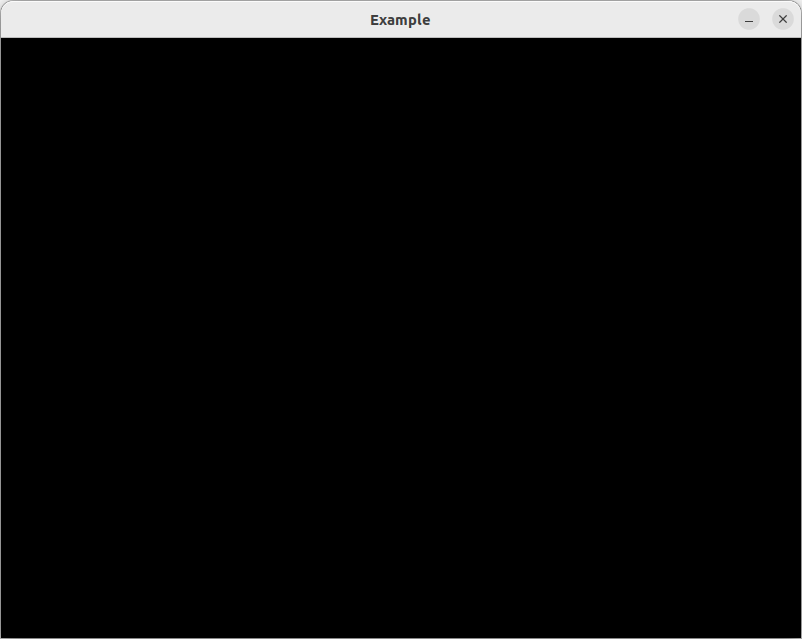
\includegraphics[width=0.5\linewidth]{figs/window.png}
\end{frame}

\subsection{Drawing setup}
\begin{frame}{Arcade}{Drawing setup (I)}
	\begin{columns}
 	   \column{0.80\textwidth}
		\vspace{-0.2cm}
		\begin{exampleblock}{drawing.py}
		\vspace{-0.2cm}
		\lstinputlisting[numbers=left]{code/drawing.py}
		\vspace{-0.2cm}
		\end{exampleblock}
	\end{columns}
\end{frame}

\begin{frame}{Arcade}{Drawing setup (II)}
	\centering 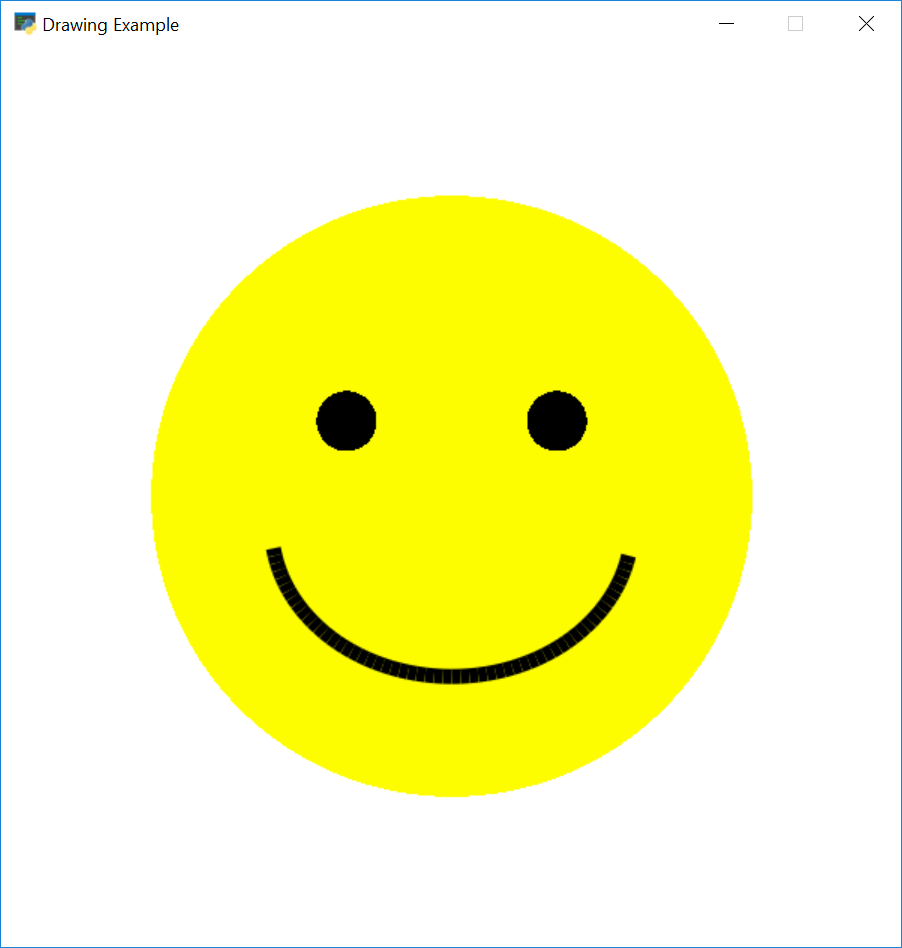
\includegraphics[width=0.5\linewidth]{figs/smile.png}
    \bigskip

    \href{https://api.arcade.academy/en/latest/examples/happy_face.html}{(Source code)}
\end{frame}

\subsection{Drawing}
\begin{frame}{Arcade}{Drawing (I)}
	\begin{columns}
 	   \column{\textwidth}
		\vspace{-0.2cm}
		\begin{exampleblock}{smile.py}
		\vspace{-0.2cm}
		\lstinputlisting[numbers=left]{code/smile.py}
		\vspace{-0.2cm}
		\end{exampleblock}
	\end{columns}
\end{frame}

\begin{frame}{Arcade}{Drawing (II)}
	\centering 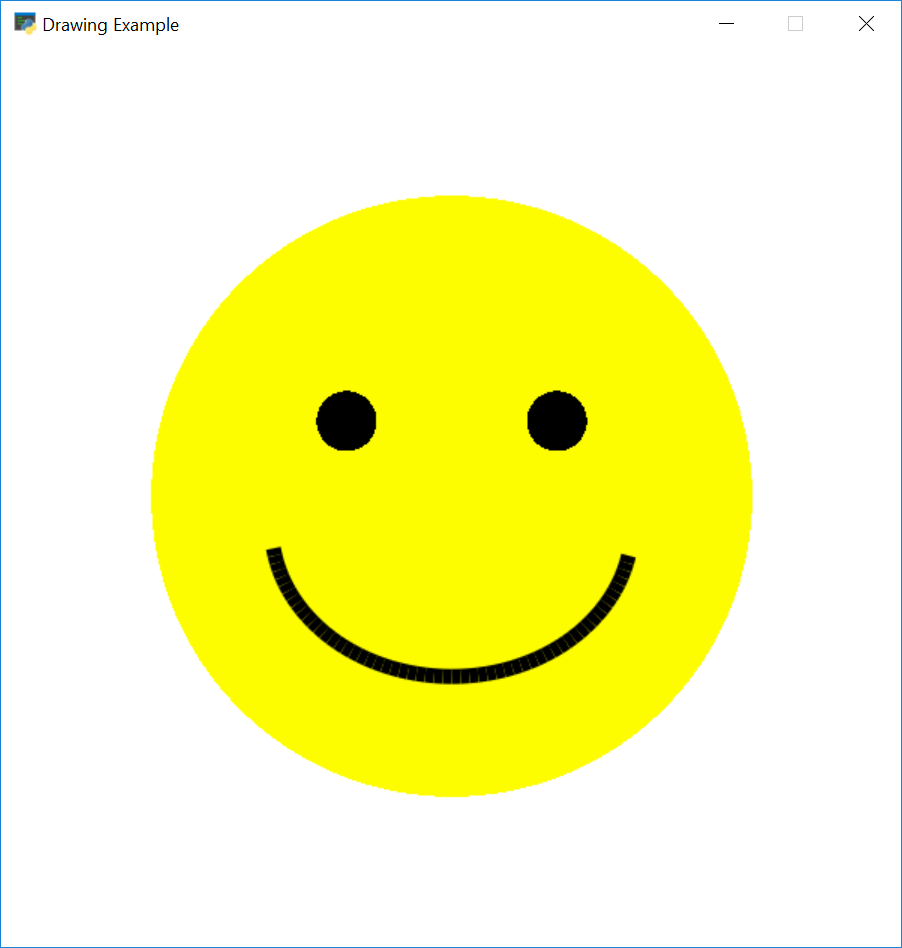
\includegraphics[width=0.5\linewidth]{figs/smile.png}
    \bigskip

    \href{https://api.arcade.academy/en/latest/examples/happy_face.html}{(Source code)}
\end{frame}

\subsection{Drawing primitives}
\begin{frame}{Arcade}{Drawing primitives (I)}
	\centering 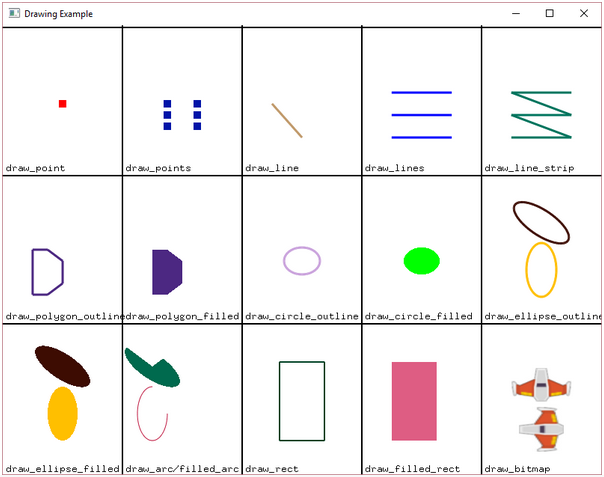
\includegraphics[width=0.7\linewidth]{figs/primitives.png} \\
    \bigskip

    \href{https://api.arcade.academy/en/latest/examples/drawing_primitives.html}{(Source code)}
\end{frame}

\begin{frame}[shrink]{Arcade}{Drawing primitives (II)}
  	\begin{multicols}{2}
		\texttt{draw\_rectangle\_filled()}\\	
		\texttt{draw\_rectangle\_outline()}\\
		\texttt{draw\_lrtb\_rectangle\_filled()}\\
		\texttt{draw\_lrtb\_rectangle\_outline()}\\
		\texttt{draw\_xywh\_rectangle\_filled()}\\
		\texttt{draw\_xywh\_rectangle\_outline()}\\
		\texttt{ }\\
		\texttt{draw\_polygon\_filled()}\\
		\texttt{draw\_polygon\_outline()}\\
		\texttt{ }\\
		\texttt{load\_texture()}\\
		\texttt{draw\_texture\_rectangle()}\\
		\texttt{draw\_xywh\_rectangle\_textured()}\\
		\texttt{ }\\
		\texttt{draw\_triangle\_filled()}\\
		\texttt{draw\_triangle\_outline()}\\
		\texttt{ }\\
		\texttt{draw\_arc\_filled()}\\
		\texttt{draw\_arc\_outline()}\\
		\texttt{ }\\
		\texttt{draw\_circle\_filled()}\\
		\texttt{draw\_circle\_outline()}\\
		\texttt{ }\\
		\texttt{draw\_ellipse\_filled()}\\
		\texttt{draw\_ellipse\_outline()}\\
		\texttt{ }\\
		\texttt{draw\_line()}\\
		\texttt{draw\_line\_strip()}\\
		\texttt{draw\_lines()}\\
		\texttt{ }\\
		\texttt{draw\_point()}\\
		\texttt{draw\_points()}
	\end{multicols}
\end{frame}

\subsection{Colors}
\begin{frame}{Arcade}{Colors}
	How can I know which colors has Arcade available?
	\begin{itemize}
		\item The reference API is your friend!
		\item \href{https://api.arcade.academy/en/latest/arcade.color.html}{(\texttt{arcade.color} reference documentation)}
	\end{itemize}


\end{frame}

\end{document}
